% Tamanho do texto, tipo de papel e documento
\documentclass[12pt,a4paper]{article}

% PACOTES
% Padrão
\usepackage[utf8]{inputenc}
\usepackage{amsmath}
\usepackage{amsfonts}
\usepackage{amssymb}

% Pacotes para alterar fonte
\usepackage[T1]{fontenc}
\usepackage{uarial}
% Personaliza lista de itens
\usepackage{enumitem}
% Muda fonte dos "captions"
\usepackage[font=small]{caption}
% Permite adicionar imagens
\usepackage{graphicx}
% Pacote para referências
%\usepackage{csquotes}
% Coloca alguns termos do artigo em português (figura, tabela)
\usepackage[brazilian]{babel}
% Permite alterar distância entre linhas
\usepackage{setspace}
% Colocando indentação em todos os parágrafos (por default o primeiro parágrafo da seção não tem)
\usepackage{indentfirst}
% Margens nas páginas
\usepackage[top=3cm, left=3cm, bottom=2cm, right=2cm]{geometry}
% Links do sumário para as respectivas páginas
\usepackage[colorlinks=true,linkcolor=black]{hyperref}
% Visualização de códigos no meio do texto
\usepackage{listings}
% Cores no código
\usepackage{color}
% Para inserir URLs
\usepackage{hyperref}
\makeatletter
\g@addto@macro{\UrlBreaks}{\UrlOrds}
\makeatother
% Para impedir as imagens de irem para lugares que não devem
\usepackage{placeins}
% Usado para centralizar verticalmente em tabelas
\usepackage{array}
% Mesclar células de uma mesma coluna no tabular
\usepackage{multirow}
% Fórmulas
\usepackage{mathtools}


% CONFIGURAÇÃO DE VARIÁVEIS
% Mostra numero da pagina no canto superior direito
\pagestyle{myheadings}
% Indentação dos parágrafos
\parindent 30pt
% Distância entre linhas
\onehalfspacing
% Acessando comandos internos
\makeatletter
	% Colocando espaço de "um espaço" entre o número e o título da seção (default é espaço de 1 quad (1em))
	\renewcommand{\@seccntformat}[1]{\csname the#1\endcsname\ }
	% Deixa os itens do sumário com pontos
	\renewcommand*\l@section{\@dottedtocline{1}{1.5em}{3.0em}}
	% Remove indentação no sumário
	\renewcommand*\l@subsection{\@dottedtocline{2}{1.5em}{3.0em}}
	\renewcommand*\l@subsubsection{\@dottedtocline{3}{1.5em}{3.0em}}
	% Criando linhas mais grossas nas tabelas
	\newcommand{\thickhline}{%
    	\noalign {\ifnum 0=`}\fi \hrule height 1pt
    	\futurelet \reserved@a \@xhline
	}
	\newcolumntype{?}{@{\hskip\tabcolsep\vrule width 1pt\hskip\tabcolsep}}
\makeatother
% Editando títulos dos índices
\addto\captionsbrazilian{
	\renewcommand{\listfigurename}{\centering LISTA DE FIGURAS}
	\renewcommand{\listtablename}{\centering LISTA DE TABELAS}
	\renewcommand{\contentsname}{\centering SUMÁRIO}
}
% Escolhendo a fonte 
\renewcommand{\familydefault}{\sfdefault}
% Estilo de listas
\renewcommand{\theenumi}{\alph{enumi}}
% Cor da URL
\hypersetup{urlcolor=black}
% Fonte da URL
\urlstyle{sf}


% INFORMAÇÕES DO TRABALHO
\author{MATEUS GONÇALEZ ETTO}
\title{UTILIZAÇÃO DE INTELIGÊNCIA ARTIFICIAL EM JOGO RPG}
\date{\today}


% COMANDOS PERSONALIZADOS
% Fonte da imagem
\newcommand{\source}[1]{\small Fonte: {#1}}
% Citações longas
\def\longcitation{\list{}{\vspace{-6mm} \leftmargin4.0cm \singlespace \small}\item[]}
\let\endlongcitation=\endlist
% Capa: objetivo do trabalho
\def\articleobjective{\list{}{\vspace{1.5cm} \leftmargin7.0cm \singlespace \small}\item[]}
\let\endarticleobjective=\endlist
% Código C#
\definecolor{codegreen}{rgb}{0,0.6,0}
\definecolor{codelightgreen}{rgb}{0.5,1,0.5}
\definecolor{codepurple}{rgb}{0.62,0,0.84}
\definecolor{codeblue}{rgb}{0,0,1}
\definecolor{backcolour}{rgb}{0.95,0.95,0.92}
\lstdefinestyle{mystyle}{
    backgroundcolor=\color{backcolour},   
    commentstyle=\color{codegreen},
    keywordstyle=\color{codeblue},
    numberstyle=\tiny\color{codelightgreen},
    stringstyle=\color{codepurple},
    basicstyle=\footnotesize,
    breakatwhitespace=false,
    breaklines=true,
    captionpos=b,
    keepspaces=true,
    numbers=left,
    numbersep=5pt,
    showspaces=false,
    showstringspaces=false,
    showtabs=false,
    tabsize=2
}
\lstset{literate=
  {á}{{\'a}}1 {é}{{\'e}}1 {í}{{\'i}}1 {ó}{{\'o}}1 {ú}{{\'u}}1
  {Á}{{\'A}}1 {É}{{\'E}}1 {Í}{{\'I}}1 {Ó}{{\'O}}1 {Ú}{{\'U}}1
  {à}{{\`a}}1 {è}{{\`e}}1 {ì}{{\`i}}1 {ò}{{\`o}}1 {ù}{{\`u}}1
  {À}{{\`A}}1 {È}{{\'E}}1 {Ì}{{\`I}}1 {Ò}{{\`O}}1 {Ù}{{\`U}}1
  {ä}{{\"a}}1 {ë}{{\"e}}1 {ï}{{\"i}}1 {ö}{{\"o}}1 {ü}{{\"u}}1
  {Ä}{{\"A}}1 {Ë}{{\"E}}1 {Ï}{{\"I}}1 {Ö}{{\"O}}1 {Ü}{{\"U}}1
  {â}{{\^a}}1 {ê}{{\^e}}1 {î}{{\^i}}1 {ô}{{\^o}}1 {û}{{\^u}}1
  {Â}{{\^A}}1 {Ê}{{\^E}}1 {Î}{{\^I}}1 {Ô}{{\^O}}1 {Û}{{\^U}}1
  {œ}{{\oe}}1 {Œ}{{\OE}}1 {æ}{{\ae}}1 {Æ}{{\AE}}1 {ß}{{\ss}}1
  {ű}{{\H{u}}}1 {Ű}{{\H{U}}}1 {ő}{{\H{o}}}1 {Ő}{{\H{O}}}1
  {ç}{{\c c}}1 {Ç}{{\c C}}1 {ø}{{\o}}1 {å}{{\r a}}1 {Å}{{\r A}}1
  {€}{{\EUR}}1 {£}{{\pounds}}1
}
\lstset{style=mystyle}


% INICIO DO ARTIGO
\begin{document}

% CAPA - INÍCIO
\thispagestyle{empty} % Oculta o número da página
\begin{center}
\makeatletter
	\textbf{UNIVERSIDADE ESTADUAL PAULISTA}\\
	\textbf{FACULDADE DE CIÊNCIAS}\\
	\textbf{DEPARTAMENTO DE COMPUTAÇÃO}\\
	\textbf{BACHARELADO EM CIÊNCIA DA COMPUTAÇÃO}\\

	\vspace{4.5cm} % Adicionando espaço extra
	\textbf{\@author}

	\vspace{4.5cm} % Adicionando espaço extra
	\textbf{\large \@title}
	
	\vspace*{\fill} % Adicionando espaço para escrever em baixo
	BAURU – SP\\
	\the\year
\makeatother
\end{center}
% CAPA - FIM

% FOLHA DE ROSTO - INÍCIO
\newpage % Coloca o conteúdo numa nova página
\thispagestyle{empty} % Oculta o número da página
\begin{center}
\makeatletter
	\textbf{\@author}

	\vspace{4.5cm} % Adicionando espaço extra
	\textbf{\large \@title}
\makeatother
\end{center}

\begin{articleobjective}
	Trabalho de Conclusão de Curso de graduação apresentado à disciplina Projeto e Implementação de Sistemas do curso de Bacharelado em Ciência da Computação da Faculdade de Ciências da Universidade Estadual Paulista "Júlio de Mesquita Filho"{} como requisito para obtenção do título de Bacharel em Ciência da Computação.
	
	\vspace{1.0cm} % Adicionando espaço extra
	Orientadora: Profa. Dra. Simone das Graças Domingues Prado
\end{articleobjective}

\begin{center}
	\vspace*{\fill} % Adicionando espaço para escrever em baixo
	BAURU – SP\\
	\the\year
\end{center}
% FOLHA DE ROSTO - FIM

% FOLHA DE APROVAÇÃO - INÍCIO
\newpage % Coloca o conteúdo numa nova página
\thispagestyle{empty} % Oculta o número da página
\begin{center}
\makeatletter
	\textbf{\@author}

	\vspace{3.0cm} % Adicionando espaço extra
	\textbf{\large \@title}
\makeatother
\end{center}

\begin{articleobjective}
	Trabalho de Conclusão de Curso de graduação apresentado à disciplina Projeto e Implementação de Sistemas do curso de Bacharelado em Ciência da Computação da Faculdade de Ciências da Universidade Estadual Paulista "Júlio de Mesquita Filho"{} como requisito para obtenção do título de Bacharel em Ciência da Computação.
\end{articleobjective}

\begin{center}
	\vspace{1.0cm}
	BANCA EXAMINADORA\\
	
	\vspace{1.0cm}
	\underline{\hspace{8cm}}\\
	Profa. Dra. Simone das Graças Domingues Prado\\
	\vspace{1.0cm}
	\underline{\hspace{8cm}}\\
	(Nome do segundo membro da Banca Examinadora)\\
	\vspace{1.0cm}
	\underline{\hspace{8cm}}\\
	(Nome do terceiro membro da Banca Examinadora)

	\vspace*{\fill} % Adicionando espaço para escrever em baixo
	Bauru, \underline{\hspace{1cm}} de \underline{\hspace{3cm}} de \underline{\hspace{1.5cm}}
\end{center}
% FOLHA DE APROVAÇÃO - FIM

% RESUMO - INÍCIO
\newpage % Coloca o conteúdo numa nova página
\thispagestyle{empty} % Oculta o número da página
\section*{\hfil RESUMO} % \hfil centraliza o título
	\singlespace
	\noindent
	Este projeto trata-se da criação de um protótipo de jogo no estilo RPG em turnos,
	em conjunto com a criação de uma Inteligência Artificial capaz de controlar os personagens,
	assim como de aprender a controlá-los melhor com treinamento.
	Para a criação da Inteligência Artificial,
	foram usados conceitos de Redes Neurais Artificiais e Algorítimo Genético,
	e para a criação do jogo e seus scripts
	foi usado o motor de jogo Unity.
	
	\vspace{0.8cm}
	\noindent
	\textbf{PALAVRAS-CHAVE:} Inteligência Artificial, Unity, jogo RPG
% RESUMO - FIM

\onehalfspacing

% ABSTRACT - INÍCIO
\newpage % Coloca o conteúdo numa nova página
\thispagestyle{empty} % Oculta o número da página
\section*{\hfil ABSTRACT} % \hfil centraliza o título
	\singlespace
	\noindent
	This project comes to creating a turn-based RPG game prototype,
	in conjunction with an Artificial Intelligence that is able to control the characters
	as well as to learn how to control them better with training.
	For the creation of the Artificial Intelligence,
	concepts of Artificial Neural Networks and Genetic Algorithm were used,
	and for the creation of the game and its scripts,
	the Unity game engine was used.
	
	\vspace{0.8cm}
	\noindent
	\textbf{KEY-WORDS:} Artificial Intelligence, Unity, RPG game
% ABSTRACT - FIM

\onehalfspacing

% LISTA DE FIGURAS - INÍCIO
\newpage % Coloca o conteúdo numa nova página
\thispagestyle{empty} % Oculta o número da página
\listoffigures % Cria a lista de figuras
% LISTA DE FIGURAS - FIM

% LISTA DE TABELAS - INÍCIO
\newpage % Coloca o conteúdo numa nova página
\thispagestyle{empty} % Oculta o número da página
\listoftables % Cria a lista de tabelas
% LISTA DE TABELAS - FIM

% SUMÁRIO - INÍCIO
\newpage % Coloca o conteúdo numa nova página
\thispagestyle{empty} % Oculta o número da página
\tableofcontents % Cria o Sumário
% SUMÁRIO - FIM

% INTRODUÇÃO - INÍCIO
\newpage % Coloca o conteúdo numa nova página
\section{INTRODUÇÃO}
	Há ainda muitas pessoas que acreditam que jogos eletrônicos são para crianças ou pessoas desocupadas.
	Talvez isso fosse verdade no milênio passado, mas a realidade vem se mostrando ser bem diferente.
	
	De acordo com uma pesquisa da SuperData,
	o mercado de jogos cresceu 8\% de 2014 a 2015,
	com 61 bilhões de dólares circulando nesta indústria (CNBC, 2016).
	Em 2014, o valor da indústria de jogos já havia ultrapassado o da indústria de música em 20 bilhões,
	e está chegando ao da indústria do filmes (NYTIMES, 2014).
	
	Então é fato, a indústria de jogos está movendo bilhões de dólares pelo mundo,
	já passou do de música e não para de crescer.
	Como diz o gerente de produto da Eletronic Sports League, James Lampkin:
	%no artigo da New York Times:
	"Isto está se expandindo fora de controle"{}
	(NYTIMES, 2014, tradução nossa).
	Tais palavras explicam muito bem o estado atual do mercado de jogos.
	
	E não é só nas vendas de jogos e consoles,
	existem muitos torneios de jogos ocorrendo pelo mundo,
	surgindo uma nova categoria de profissionais que,
	em poucos anos atrás era inimaginável, senão motivo de piada,
	que é a categoria de jogador profissional de jogo eletrônico.
	A área de trabalho já existe e é chamada de Esporte Eletrônico (NYTIMES, 2014).
	
	E mesmo nestes torneios, não é por pouco dinheiro que os jogadores se enfrentam.
	No Campeonato Mundial de 2015 (o quinto da série) de League of Legends,
	foi oferecido 1 milhão de dólares para a equipe vencedora mundial do jogo,
	como pode ser visto nas regras do campeonato\footnote{Regras: \url{https://riot-web-static.s3.amazonaws.com/lolesports/Rule\%20Sets/2015\%20Revised\%20World\%20Championship\%20Rule\%20Set\%20Version\%201\_01.pdf}}.
	
	Os prêmios não param por aí.
	O jogo Dota 2 distribuiu 11 milhões de dólares para os 10 melhores do mundo,
	sendo 5 milhões para os campeões,
	se tornando assim o maior prêmio já oferecido em um torneio de jogo eletrônico (NYTIMES, 2014).
	
	E tem muita gente para assistir a estes campeonatos.
	Nos dados mostrados pela Riot\footnote{Dados disponíveis em: \url{http://www.lolesports.com/en_US/articles/worlds-2015-viewership}}
	sobre o Campeonato Mundial de 2015,
	houveram 334 milhões de telespectadores "únicos"{} durante as 4 semanas do torneio,
	somando 360 milhões de horas de visualizações das partidas ao vivo.
	
	Mas a área de jogos não está chamando apenas a atenção do mercado,
	mas também a de pesquisadores.
	Um exemplo é o desenvolvimento e aplicação de técnicas de Inteligência Artificial (IA) em jogos,
	que de acordo com especialistas,
	existem áreas dentro de IA em jogos que ainda estão inexplorados (YANNAKAKIS; TOGELIUS, 2014).
	
	Em 2007, foi montada pela AiGameDev uma lista dos 10 jogos com Inteligência Artificial mais influentes.
	Um exemplo é um jogo chamado Creatures,
	que implementou aprendizado de máquina em uma simulação interativa
	ao usar Redes Neurais nas criaturas do jogo.
	Outro exemplo é o Halo,
	o jogo que implementou pela primeira vez a "árvore de condutas",
	tecnologia que ficou muito popular na indústria de jogos (AIGAMEDEV, 2007).
	
	Um exemplo de IA em jogo que é descrito em detalhes é o F.E.A.R.,
	um jogo FPS em primeira pessoa
	que criou um sistema dinâmico, coordenado, interessante e desafiador.
	Isto foi feito utilizando um sistema chamado Goal Oriented Action Planning (Planejamento de Ações Orientado a Objetivo),
	que foi construído junto de duas técnicas: Algoritmo A* e Máquina de Estados Finitos.
	Os NPCs possuem uma lista de objetivos,
	então durante o jogo eles buscam o plano que irá completar o objetivo com maior prioridade.
	O planejamento feito é similar ao STRIPS,
	tendo-se a situação atual e quais são as ações necessárias para cumprir o objetivo.
	Além disto, foi implementado uma extensão da conduta individual dos NPCs
	com uma conduta em equipe.
	No entanto, como a conduta dos NPCs foi criada para minimizar a ameaça a si mesmo,
	os extintos básicos do NPC podem sobrescrever a conduta de equipe
	caso a segunda opção seja muito arriscada para si mesmo (ORKIN, 2006).
	
	Percebe-se, desta forma, que a área de jogos está muito ativa e em pleno crescimento,
	tanto no mercado quando em pesquisas.
	Existem áreas inexploradas de IA em jogos,
	com novas fronteiras a serem exploradas.
	Com isto em mente, este trabalho foi desenvolvido,
	%aumentando o número de trabalhos que estão explorando esta área,
	e espera-se contribuir com a comunidade acadêmica e/ou mercado de alguma forma.

	\FloatBarrier
	\subsection{Objetivos do Trabalho}
	
		\FloatBarrier
		\subsubsection{Objetivo Geral}
			Produzir um jogo RPG em turnos que implementa conceitos avançados de Inteligência Artificial,
			sendo esta inteligência capaz de tomar decisões de forma autônoma sobre o que deve fazer,
			assim como ser capaz de aprender a tomar melhores decisões por meio de treinamento.
		
		\FloatBarrier
		\subsubsection{Objetivos Específicos}
			\begin{enumerate}[noitemsep]
				\item Criar um jogo RPG razoavelmente complexo.
				\item Criar uma Inteligência Artificial capaz de jogar o jogo tão bem quanto um ser humano.
				\item Criar uma Inteligência Artificial capaz de aprender conforme joga.
			\end{enumerate}			
	
	\FloatBarrier
	\subsection{Organização da Monografia}
		Este trabalho está dividido em 5 seções, sendo esta seção (Introdução) a primeira. As outras seções são:
		\begin{itemize}[noitemsep]
     		\item Seção 2, \textbf{Ferramentas Utilizadas:} apresentação das ferramentas utilizadas para o desenvolvimento do projeto proposto no trabalho.
     		\item Seção 3, \textbf{Conceitos:} explicação das teorias de Inteligência Artificial e Algoritmo Genético usadas para desenvolver o trabalho.
     		\item Seção 4, \textbf{O Jogo:} descrição em detalhes do jogo, suas variáveis, e de sua implementação.
     		\item Seção 5, \textbf{Resultados:} apresentação dos resultados obtidos no trabalho.
  	 	\end{itemize}
% INTRODUÇÃO - FIM

% DESENVOLVIMENTO - INÍCIO
\FloatBarrier
\newpage % Coloca o conteúdo numa nova página
\section{FERRAMENTAS UTILIZADAS}

	\FloatBarrier
	\subsection{Unity}
		A Unity é um motor de jogo multiplataforma que permite a criação de jogos 2D ou 3D.
		Possui uma interface gráfica que permite desenvolver jogos com facilidade,
		além de ter muitos serviços integrados que aceleram o processo de desenvolvimento.
		As linguagens de programação que podem ser usadas são UnityScript e C\#
		(UNITY, 2016a).
		
		Com mais de 200 jogos na lista de jogos em destaque que foram criados na Unity,
		um dos exemplos que pode-se citar é o \textit{Sky Force},
		um jogo no estilo de ação, missões e "shooter",
		e que está disponível na App Store e Google Play.
		Outro exemplo é o \textit{The Uncertain},
		do qual o jogador é um robô e
		deve resolver quebra-cabeças em uma aventura.
		O jogo está disponível na \textit{Steam}
		(UNITY, 2016b).
		
		O editor da Unity também é extensível, sendo possível implementar funcionalidades ainda não existentes
		(UNITY, 2016a).
		Um exemplo de extensão é o \textit{Rival Theory},
		que implementa vários conceitos de Inteligência Artificial,
		desde funcionalidades básicas como \textit{pathfinding},
		condutas de patrulha, esconder, atacar, seguir, vaguear,
		até conceitos mais complicados como percepção e árvore de condutas
		(RIVAL THEORY, 2015).
		
		\FloatBarrier
		\subsubsection{Interface}
			A interface da Unity é composta por vários painéis chamados \textit{views},
			que podem ser rearranjados, agrupados, separados e fixados
			(UNITY, 2016c).
			O arranjamento padrão das janelas permite o acesso às janelas mais comuns,
			e pode ser visto na Figura \ref{fig:interfaceUnity} a seguir:
			
			\begin{figure}[ht!]
				\caption{A interface padrão da Unity}
				\centering
				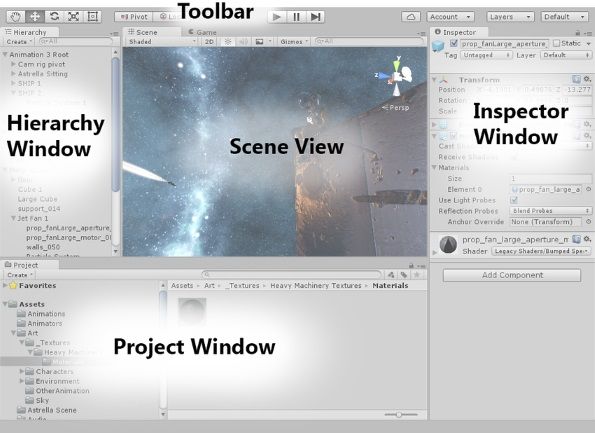
\includegraphics[scale=0.5]{InterfaceUnity.jpg}\\
				\vspace{0.5mm}
				\source{Unity.}
				\label{fig:interfaceUnity}
			\end{figure}	
			
			A descrição de cada painel pode ser vista na Tabela \ref{tab:unity} a seguir:
			
			\begin{table}[ht]
				\caption{Descrição dos painéis na Unity}
				\centering
				\small
				\renewcommand{\arraystretch}{1.2} % Aumenta espaçamento vertical
				\begin{tabular}{m{3.1cm} m{11.9cm}}
					\hline 
					Project Window & Exibe a biblioteca de Assets que estão disponíveis para uso no projeto. Ao importar os Assets no projeto, eles aparecerão aqui. \\ 
					\hline 
					Scene View & Permite navegar visualmente e editar a cena. A Scene View pode mostrar em perspectiva 3D ou 2D, dependendo do tipo de projeto que está sendo trabalhando. \\ 
					\hline 
					Hierarchy Window & É uma representação de texto hierárquica de cada objeto na cena. Cada item na cena tem uma entrada na hierarquia, de forma que as duas janelas estão inerentemente conectadas. A hierarquia revela a estrutura da forma como os objectos estão ligados um ao outro. \\ 
					\hline 
					Inspector Window & Permite visualizar e editar todas as propriedades do objeto selecionado. Como diferentes tipos de objetos têm diferentes conjuntos de propriedades, o layout e conteúdo da janela do Inspector pode variar. \\ 
					\hline 
					Toolbar & Fornece acesso aos recursos de trabalho mais essenciais. À esquerda estão as ferramentas básicas para manipular a Scene View e os objetos dentro dela. No centro estão os controles de play, pause e step. Os botões à direita dará acesso aos Serviços da Unity Cloud e da Conta Unity, seguido pelo menu de visibilidade dos layers e, finalmente, o menu de layout do editor (que fornece alguns layouts alternativos para as janelas do editor, e permite salvar um layout customizado). \\ 
					\hline 
				\end{tabular}\\
				\vspace{3mm}
				\source{Unity.}
				\label{tab:unity}
			\end{table}
			
			Os objetos contidos na cena do projeto são chamados de \textit{GameObject},
			sendo que suas características podem ser alteradas por Componentes anexados a ele.
			A Unity possui vários Componentes prontos,
			no entanto é possível criar novos usando as linguagens de programação do qual se dá suporte (C\# e UnityScript).
			Tais Componentes são chamados de Scripts,
			e eles permitem disparar eventos,
			modificar as propriedades de outros Componentes ou do próprio \textit{GameObject} durante o jogo,
			e a interação com o jogador.
			(UNITY, 2016d).

	\FloatBarrier
	\subsection{Visual Studio}
		O Visual Studio é um Ambiente de Desenvolvimento Integrado (IDE) usado para a criação de aplicativos para Windows, Android, iOS, aplicações Web e serviços de nuvem.
		Com ele é possível programar em C\#, Visual Basic, F\#, C++, HTML, JavaScript e Python, dentre outras linguagens de programação. (MICROSOFT, 2016)
		
		A integração do Visual Studio com a Unity, usando C\#, ocorre com a adição do \textit{namespace} UnityEngine ao script,
		%(com o código "using UnityEngine"),
		liberando a utilização da classe \textit{MonoBehaviour},
		da qual possui implementado funcionalidades e funções internas da Unity.
		Para utilizar a classe \textit{MonoBehaviour} nos scripts criados,
		basta estender a classe criada com a \textit{MonoBehaviour} (UNITY, 2016d).
		Desta forma, o cabeçalho do script fica como no código a seguir:
		
		\begin{lstlisting}[language=C++]
using UnityEngine;

public class nomeDaClasse : MonoBehaviour
{
	// Código da classe
}\end{lstlisting}
		
		Com isto feito, é possível utilizar uma das principais vantagens do Visual Studio,
		que é o \textit{AutoComplete}.
		Ou seja, funções internas da Unity, como as do GameObject, aparecem em uma lista conforme se vai digitando,
		facilitando muito a programação do script.
		
		Além da integração com a Unity,
		ainda é possível utilizar as bibliotecas próprias do C\#,
		como bibliotecas matemáticas, acesso à arquivo e listas.
		
		Na \textit{Figura \ref{fig:exvs}} a seguir, é possível ver um exemplo de classe criada no Visual Studio que foi usada neste projeto:
		
		\begin{figure}[ht!]
			\caption{Exemplo de classe no Visual Studio}
			\centering
			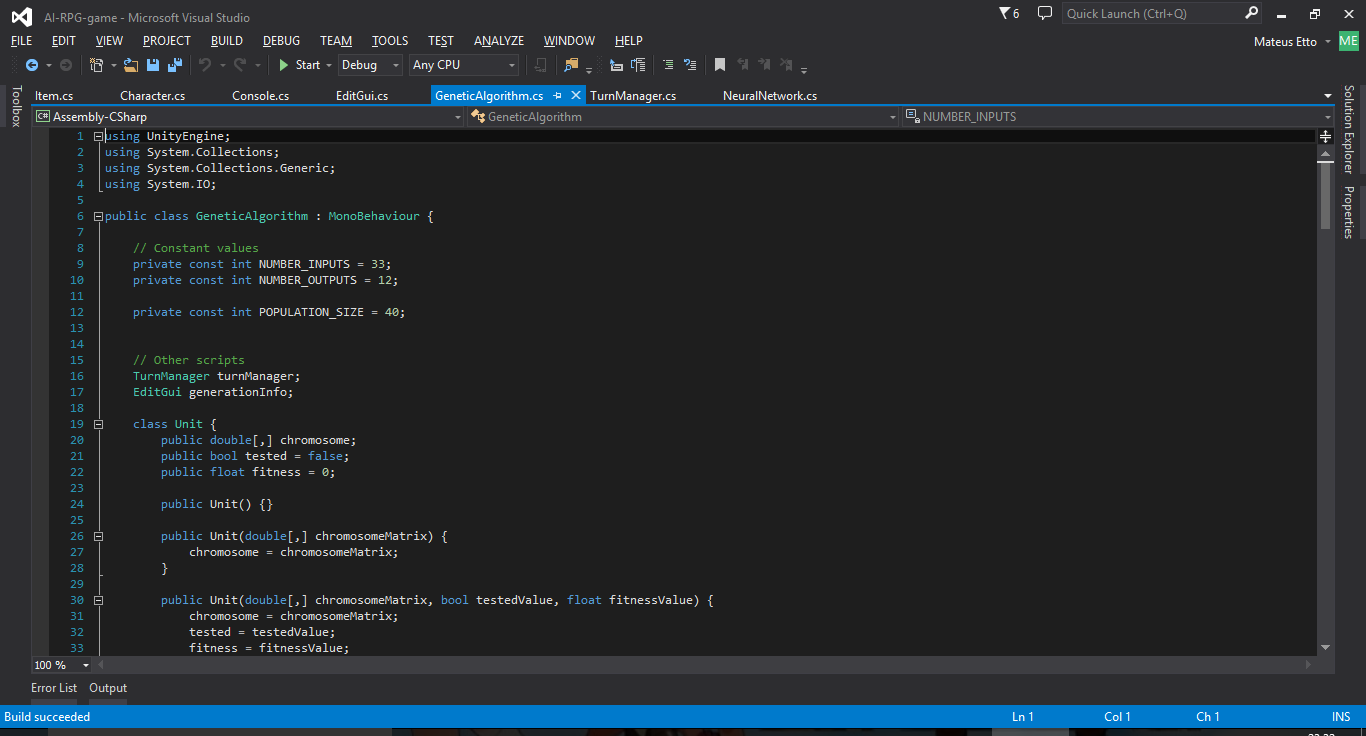
\includegraphics[scale=0.4]{InterfaceVisualStudio.png}\\
			\vspace{0.5mm}
			\source{Elaborado pelo autor.}
			\label{fig:exvs}
		\end{figure}
		
		Nota-se que no script de Algoritmo Genético, além do \textit{UnityEngine} e outras duas bibliotecas básicas do C\#,
		também foi utilizada o \textit{System.IO}, uma biblioteca para Leitura e Escrita de Arquivo.
		Qualquer outro script criado para funcionar na Unity tem este padrão.

\FloatBarrier
\newpage % Coloca o conteúdo numa nova página	
\section{CONCEITOS}

	Nesta seção será descrito dois conceitos que foram amplamente utilizados neste trabalho,
	que são Redes Neurais Artificiais (RNA) e Algoritmo Genético (AG).
	Apesar de ser possível descrever várias variações de aplicação desses conceitos,
	será explicado apenas a essência deles,
	e o que foi necessário para desenvolver este trabalho.

	\FloatBarrier
	\subsection{Redes Neurais Artificiais}
	% 1 Definição
	As Redes Neurais Artificiais são uma família de modelos inspirados no funcionamento do cérebro humano,
	sendo que a "baixo nível"{} procuram imitar o que acontece nos neurônios.
	São usadas para estimar ou aproximar funções que dependam de um grande número de entradas.
	
	\subsubsection{Funcionamento}
	% 2 Arquitetura
	% 2.1 Funções de entrada e ativação
	A unidade em uma RNA é o neurônio.
	O neurônio recebe estímulos, que na RNA são números reais.
	Recebendo os vários estímulos, o neurônio faz uma operação com todos os números recebidos,
	que normalmente é um somatório.
	Esta é a função de entrada.
	
	Após aplicar a função de entrada em todos os estímulos,
	é obtido um único valor.
	Este valor, então, é processado por uma função de ativação.
	Existem várias funções de ativação que podem ser utilizadas,
	e pode-se ver alguns exemplos na Figura \ref{fig:activationFunctions}.
	
	\begin{figure}[ht!]
		\caption{Funções de Ativação comuns em uma RNA}
		\centering
		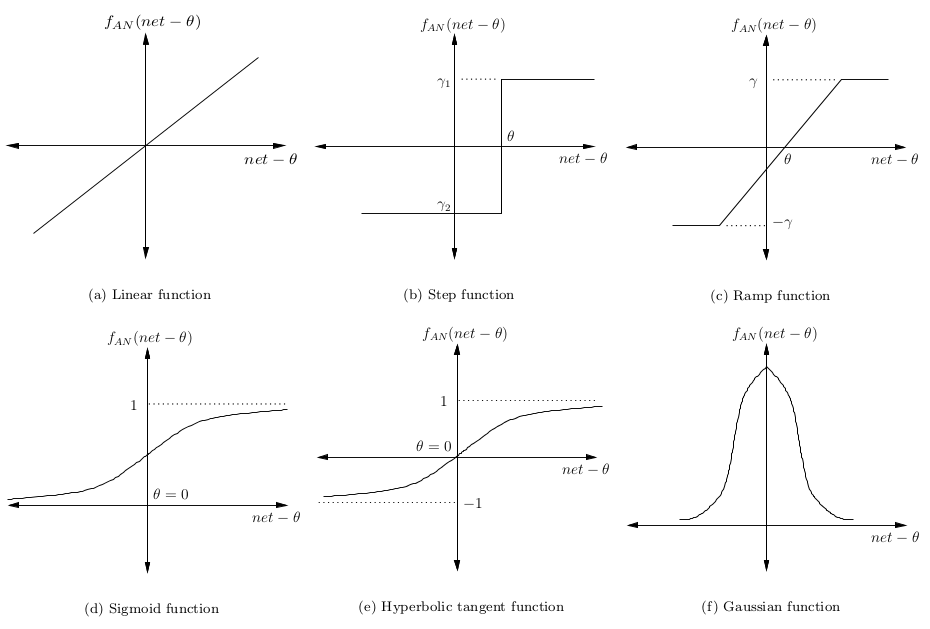
\includegraphics[scale=0.39]{ActivationFunctions.png}\\
		\vspace{0.5mm}
		\source{Turing Finance.}
		\label{fig:activationFunctions}
	\end{figure}
	
	Diferentes funções de ativação se adequam melhor dependendo da aplicação da RNA,
	assim como a camada em que o neurônio se encontra.
	
	O resultado da função de ativação é então multiplicado por um peso,
	e passado para o próximo neurônio como um estímulo.
	
	% 2.2 Particularidades (camadas existentes, papel de cada uma)
	A arquitetura de uma RNA é formada por uma camada de entrada (input layer),
	uma camada de saída (output layer),
	e as camadas ocultas (hidden layers)
	que poderão conter de zero a muitas camadas.
	Cada camada na RNA terá \textit{n} neurônios,
	sendo \textit{n} qualquer valor maior ou igual a 1.
	Um exemplo de Rede Neural Artificial com uma camada oculta pode ser visto na Figura \ref{fig:basicnn}.
	
	\begin{figure}[ht!]
		\caption{RNA com uma camada oculta}
		\centering
		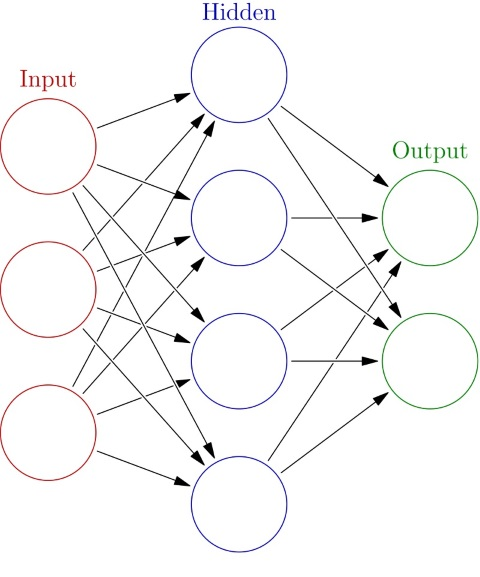
\includegraphics[scale=0.45]{BasicNN.jpg}\\
		\vspace{0.5mm}
		\source{Wikimedia.}
		\label{fig:basicnn}
	\end{figure}
	
	Como ilustrado na Figura \ref{fig:basicnn},
	cada neurônio de uma camada se conecta com todos os outros neurônios da camada seguinte.
	Existem muitas variações de arquiteturas de RNA,
	não sendo todas que seguem o padrão visto na Figura \ref{fig:basicnn},
	porém esta é a arquitetura mais "tradicional"{}.
	
	Uma Rede Neural Artificial sempre terá uma camada de entrada e uma de saída.
	No entanto, o número de camadas ocultas pode variar bastante entre um problema e outro.
	Estas camadas ocultas são explicadas como sendo "extratoras de características"{}
	(STACKEXCHANGE, 2013).
	
	Então, se o número de camadas ocultas varia,
	de que maneira pode-se determinar o número de camadas ocultas a serem utilizadas em um determinado problema?
	Caso os dados sejam linearmente separáveis,
	não é necessário nenhuma camada oculta.
	Caso contrário, se forem dados não lineares,
	uma ou mais camadas ocultas serão necessárias
	(STACKEXCHANGE, 2013).
	Quanto mais camadas ocultas forem utilizadas,
	maior a granularidade dos resultados obtidos na RNA,
	como pode ser visto na Figura \ref{fig:nnhiddenlayer}.
	
	\begin{figure}[ht!]
		\caption{Importância da camada oculta}
		\centering
		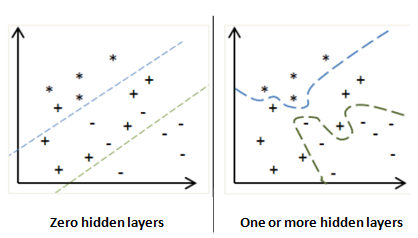
\includegraphics[scale=1.5]{HiddenLayers.png}\\
		\vspace{0.5mm}
		\source{Stackoverflow.}
		\label{fig:nnhiddenlayer}
	\end{figure}
	
	Deve-se lembrar que, apesar de muitas camadas ocultas aumentar a granularidade dos resultados,
	isto vem com um custo:
	mais tempo de processamento e
	influência no tempo de aprendizagem.
	É por este motivo que deve-se buscar a arquitetura otimizada ao problema,
	com baixo tempo de processamento e alto desempenho.
	Outro detalhe importante é a necessidade de colocar funções de ativação não-lineares nas camadas ocultas,
	uma vez que são elas que garantem a não-linearidade dos resultados
	(STACKEXCHANGE, 2013).
	
	Existem muitas discussões a respeito do número de camadas ocultas a serem usadas, caso ela seja necessária,
	mas um consenso que existe é que uma única camada é o suficiente para a maioria dos problemas
	(STACKEXCHANGE, 2013).
	
	Considerando a necessidade de colocar uma camada oculta na RNA,
	existem regras empíricas que ajudam a escolher um número de neurônios a serem colocados na camada oculta.
	Uma delas é encontrar a média do número de neurônios de entrada e de saída,
	e usar este valor como ponto de partida,
	ajustando-o então com testes
	(STACKEXCHANGE, 2013).
	
	\subsubsection{Tipos de aprendizado}
	% 3 Tipos de aprendizado (com exemplos de utilização)
	Um dos maiores atrativos de uma RNA é sua capacidade de aprender,
	e atualmente existem três paradigmas de aprendizagem:
	Aprendizado Supervisionado, Aprendizado Não-supervisionado e Aprendizado Reforçado.
	
	No Aprendizado Supervisionado,
	tem-se os dados de entrada, e infere-se os dados de saída.
	Sabendo-se estas duas informações, treina-se a RNA para que produza os resultados esperados,
	ajustando os pesos de suas conexões.
	Esta forma de aprendizagem é utilizada principalmente para duas finalidades:
	reconhecimento de padrões e regressão de funções.
	
	Dependendo da finalidade da RNA no Aprendizado Supervisionado,
	diferentes funções de ativação são recomendadas na camada de saída
	(as funções de ativação podem ser vistas na Figura \ref{fig:activationFunctions}, página \pageref{fig:activationFunctions}).
	Caso a tarefa da RNA seja de reconhecer padrões,
	as funções recomendadas são a step (b), sigmoide (d) e tangente hiperbólica (e).
	Por outro lado, se a tarefa for de regressão de uma função,
	a função linear (a) é a mais recomendada (RESEARCHGATE, 2013).
	
	No Aprendizado Não-supervisionado,
	tem-se os dados de entrada e uma função de custo a ser minimizada.
	Com o decorrer das iterações,
	os pesos da RNA serão adaptados para minimizar o custo.
	Tarefas que usam tal paradigma são os que envolvem problemas de estimativa.
	
	No Aprendizado Reforçado,
	os dados de entrada são desconhecidos,
	e o cálculo do custo é feita de maneira dinâmica.
	Os dados de entrada são gerados através das interações do RNA com o ambiente.
	Exemplos de utilização deste paradigma são
	programação dinâmica e problemas de controle.

	\FloatBarrier
	\subsection{Algoritmo Genético}
	% 1 Definição
	Algoritmo genético faz parte da computação evolutiva,
	e inspirou-se na teoria de Darwin sobre a evolução das espécies.
	É uma busca heurística usada para encontrar soluções de otimização e resolver problemas de busca.
	
	\FloatBarrier
	\subsubsection{Conceitos de AG}
	% 2 Conceitos
	% 2.1 Cromossomos
	A unidade que caracteriza um determinado indivíduo na população é o cromossomo.
	% 2.1.1 Gene
	O cromossomo é constituído de vários genes,
	que carregam uma informação ou característica de um indivíduo.
	% 2.1.2 Representação do cromossomo
	O gene pode ser representado de várias formas dentro do AG,
	sendo a mais simples delas a representação binária,
	como pode ser visto na Tabela \ref{tab:cromosome}.
	
	\begin{table}[ht]
		\caption{Representação binária de cromossomos}
		\centering
		\begin{tabular}{c c c c c c c c c c c}
			\hline 
			0 & 1 & 1 & 0 & 1 & 0 & 0 & 0 & 1 & 0 & 1\\ 
			\hline 
			1 & 0 & 1 & 0 & 0 & 1 & 1 & 0 & 0 & 1 & 0\\ 
			\hline 
		\end{tabular} \\
		\vspace{3mm}
		\source{Elaborado pelo autor.}
		\label{tab:cromosome}
	\end{table}
	
	Outras representações de cromossomos também existem.
	Por exemplo, existe a codificação por permutação,
	utilizado em problemas de ordenação.
	Neste caso, todo cromossomo é um vetor de números,
	e cada número representa uma posição.
	
	Outro exemplo é codificação por valor.
	Este valor poderá ser qualquer coisa relacionada ao problema,
	como números reais ou sequência de caracteres.
	E como último exemplo existe a codificação em árvore,
	em que cada cromossomo é uma árvore de objetos,
	como funções ou comandos em uma linguagem de programação.
	
	% 2.2 Indivíduo
	Um indivíduo no AG sempre possuirá um cromossomo.
	Este indivíduo carrega uma das possíveis soluções do problema.
	%e pode ser uma solução boa ou não.
	
	% 2.3 População
	O indivíduo faz parte de uma população.
	%Logo, pode-se dizer que uma população é um conjunto de soluções.
	% 2.3.1 Tamanho de população
	Para se resolver um problema usando AG,
	nem sempre uma população enorme irá se traduzir em uma convergência mais rápida.
	De acordo com algumas pesquisas,
	população em torno de 30 indivíduos se mostram ser eficientes,
	apesar de que outros valores possam ser melhores dependendo do problema
	(OBITKO, 1998).
	
	% 2.4 Geração
	Uma geração diz respeito à iteração do qual a população se encontra.
	Uma população nova criada a partir de uma população antiga é uma nova geração.
	Tem-se, então, várias gerações de populações diferentes (ou evoluídas).
	
	% 2.5 Avaliação
	% 2.5.1 Fitness (aptidão)
	Durante o algoritmo do AG, deve-se calcular o o fitness (nível de aptidão) de cada indivíduo da população.
	A forma de se calcular o fitness do indivíduo depende do problema,
	e este cálculo faz parte do processo de Avaliação da população,
	que pode ser visto em mais detalhes na Tabela \ref{tab:agCycle} e Figura \ref{fig:gaflow} à frente.
	
	% 2.6 Seleção
	No processo de Seleção,
	indivíduos da população são selecionados para passarem para a próxima geração ou se reproduzirem.
	A Seleção usa o valor de fitness para dar maiores chances de selecionar os indivíduos mais adaptados.
	
	% 2.6.1 Roleta
	Um método comum para se selecionar indivíduos é o método da Roleta.
	Neste método, um intervalo numérico relativo ao valor de fitness é atribuído a cada indivíduo.
	Então é sorteado aleatoriamente um valor no intervalo de todos os indivíduos.
	O indivíduo que conter o número sorteado dentro de seu intervalo é o escolhido para passar para a próxima geração ou se reproduzir.
	Percebe-se assim que indivíduos com maior fitness terão um intervalo maior e, portanto, maiores chances de serem selecionados.
	Uma ilustração do que foi descrito pode ser visto na Figura \ref{fig:roulette}.
	
	\begin{figure}[ht!]
		\centering
		\caption{Método da roleta para Seleção}
		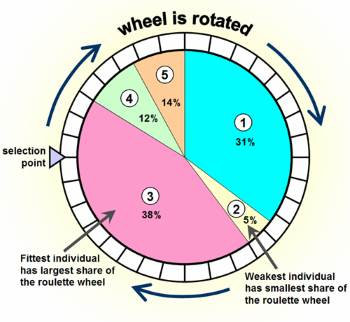
\includegraphics[scale=0.7]{Roulette.jpg}\\
		\vspace{0.5mm}
		\source{Stack overflow.}
		\label{fig:roulette}
	\end{figure}
	
	% 2.6.2 Ranking
	Outro exemplo de método de Seleção é o de Ranking.
	De forma similar ao da Roleta, é usado o valor de fitness.
	No entanto, o diferencial está no fato de ordenar os indivíduos em um ranking,
	e atribuir um intervalo numérico dependendo do ranking do indivíduo
	(quanto maior o ranking, maior o intervalo atribuído).
	
	% 2.7 Crossover
	Após a seleção existe o Crossover (ou cruzamento).
	%análogo à reprodução que se estuda em biologia.
	Se for decidido que haverá um crossover,
	informações do cromossomo de 2 indivíduos são misturados,
	criando "cromossomos filhos"{}.
	Neste processo, são selecionados pontos nos cromossomos pais,
	e os cromossomos filhos copiam do primeiro cromossomo pai até aquele ponto,
	passando então a copiar do segundo cromossomo pai.
	O crossover pode ter um único ponto ou vários pontos de crossover.
	Também existe o crossover uniforme,
	em que é copiado vários pequenos trechos de ambos os pais,
	com taxa de 50\% de se copiar de cada um deles.
	
	% 2.7.1 Taxa de Crossover
	No entanto, o crossover não necessariamente ocorre sempre.
	Existe uma probabilidade dele acontecer,
	e essa probabilidade é a taxa de crossover.
	Considerando-se, por exemplo, uma taxa de crossover de 90\%,
	tem-se que 90\% dos indivíduos selecionados passarão pelo processo de crossover,
	e que 10\% serão copiados para a nova população.
	
	% 2.8 Mutação
	Após o crossover,
	os cromossomos passam pelo processo de Mutação.
	A mutação permite a mudança de alguns genes escolhidos aleatoriamente.
	% 2.8.1 Taxa de Mutação
	A chance de ocorrer uma mutação em um determinado gene é determinado pela taxa de mutação.
	Por exemplo, se a taxa de mutação for de 1\%,
	isto significa que 1\% dos genes terão seus valores alterados.
	
	% 2.9 Elitismo
	A fim de não se perder boas soluções por causa do Crossover e Mutação,
	uma técnica muito aplicada e eficiente é a do Elitismo.
	Nesta técnica, o melhor (ou melhores) indivíduos da população são copiados sem nenhuma alteração para a próxima geração.
	
	\FloatBarrier
	\subsubsection{Processo}
	% 3 Processo
	O Algoritmo Genético mais simples de ser representado tem 5 etapas,
	em um processo que se repete até que uma determinada condição de parada seja satisfeita.
	O processo ocorre como explica a Tabela \ref{tab:agCycle} e ilustra a Figura \ref{fig:gaflow} a seguir:
	
	\begin{table}[h]
		\caption{Ciclo do Algoritmo Genético}
		\centering
		\small
		\renewcommand{\arraystretch}{1.2} % Aumenta espaçamento vertical
		\begin{tabular}{>{\centering\arraybackslash}m{3.5cm} m{11.5cm}}
			\hline 
			\textbf{Inicia População} & Gera uma população aleatória de n indivíduos. \\ 
			\hline 
			\textbf{Avaliação} & Calcula o valor de fitness de cada cromossomo na população. Se a condição de parada for satisfeita, o algoritmo acaba. \\ 
			\hline 
			\textbf{Seleção} & Seleciona 2 cromossomos de acordo com o fitness. Quanto maior o valor de fitness, maior a probabilidade de ser selecionado. \\ 
			\hline 
			\textbf{Crossover} & Copia partes dos cromossomos dos pais em cromossomos filhos, inserindo-os na nova população. \\ 
			\hline 
			\textbf{Mutação} & Aplica a probabilidade de alterar aleatoriamente os genes dos indivíduos da nova população, e retorna ao passo de Avaliação. \\ 
			\hline 
		\end{tabular}\\
		\vspace{3mm}
		\source{Elaborado pelo autor.}
		\label{tab:agCycle}
	\end{table}
	
	\begin{figure}[ht!]
		\centering
		\caption{Passo a passo do Algoritmo Genético}
		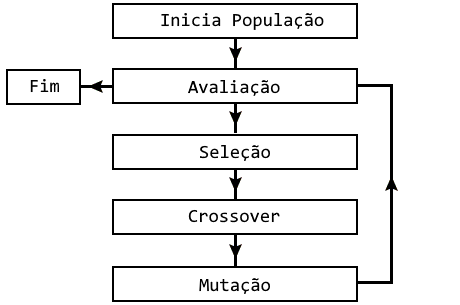
\includegraphics[scale=0.7]{GeneticAlgorithmFlow.png}\\
		\vspace{0.5mm}
		\source{Tech-Effigy.}
		\label{fig:gaflow}
	\end{figure}
	
	A condição de parada pode ocorrer por mais de um motivo.
	A melhor condição para se parar é uma boa "avaliação"{} (fitness) dos indivíduos,
	mas também é possível parar por causa de um limite de gerações ou iterações.
	
	Como é possível notar,
	a repetição das etapas de Avaliação, Seleção, Crossover e Mutação melhora gradativamente as soluções encontradas,
	sendo esta a maior motivação de se utilizar um AG.	
	
	\FloatBarrier
	\subsubsection{Exemplos de aplicação}
	% 4 Exemplos de aplicação
	Como exemplos de aplicação de AG,
	será citado
	Design Automotivo, Robótica, Otimização de rotas e Jogos.
	
	No caso de Design Automotivo,
	AGs podem auxiliar na escolha de materiais e seus formatos para a produção de veículos mais rápidos, leves, econômicos e mais seguros.
	A Figura \ref{fig:automotiveDesign} ilustra um exemplo de design de carro.
	Por se tratar de um problema de otimização,
	o AG pode encontrar várias soluções que irão ajudar o designer a projetar o veículo
	(BRAINZ, 2010).
	
	\begin{figure}[ht!]
		\centering
		\caption{Exemplo de design de carro}
		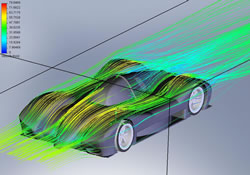
\includegraphics[scale=0.7]{AutomotiveDesign.jpg}\\
		\vspace{0.5mm}
		\source{BRAINZ.}
		\label{fig:automotiveDesign}
	\end{figure}
	
	A aplicação de AG em Robótica procura os designs de robôs mais otimizados para as suas tarefas.
	Como existem muitas "tarefas"{} que podem ser dadas aos robôs,
	diferentes designs são necessários.
	Um AG pode agilizar o processo de desenvolvimento de design de um robô,
	considerando as inúmeras variáveis e criando um design melhorado
	(BRAINZ, 2010).
	
	AGs também são capazes de encontrar boas soluções em problemas de otimização de rotas.
	As rotas podem ser de, por exemplo:
	um navio no oceano,
	um carro na estrada ou cidade,
	e dados trafegando por roteadores na internet
	(BRAINZ, 2010).
	
	E como último exemplo,
	é possível utilizar AG em jogos eletrônicos.
	O jogo The Sims permite que o jogador crie uma família e treine-a para se relacionar uns com os outros
	(BRAINZ, 2010).
	O jogo Creatures simula a vida pequenas criaturas,
	e procura ser fiel ao simular a vida deles como se fossem pequenos animais,
	criando seu "DNA"{} e características passadas geneticamente
	(AIGAMEDEV, 2007).
	
	\FloatBarrier
	\subsubsection{Variação com RNA}
	Uma diferente forma de se trabalhar com AG é juntá-la com RNA.
	Desta maneira, a RNA terá como papel o processamento de dados complexos,
	e o AG fará a busca dos pesos otimizados na RNA.
	
	Na Figura \ref{fig:nn-ag} a seguir, é possível visualizar como é implementação dos conceitos juntos.
	
	\begin{figure}[ht!]
		\centering
		\caption{RNA e AG juntos}
		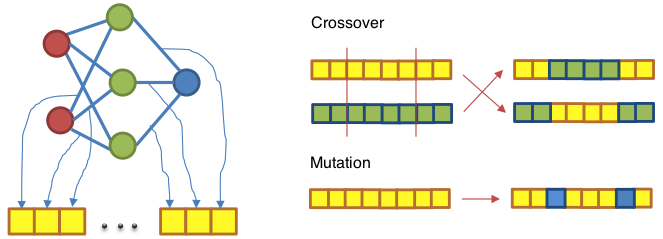
\includegraphics[scale=0.7]{NeuralNetworkIntoChromosome.png}\\
		\vspace{0.5mm}
		\source{Evo-neural-network-agents.}
		\label{fig:nn-ag}
	\end{figure}
	
	Os pesos da RNA são colocados na estrutura do cromossomo,
	e então é tratado como um cromossomo para realizar o processo do AG.
	Ao finalizar, o cromossomo retorna à RNA como pesos,
	usa-se e repete o processo.
	
	Este foi o método escolhido para a criação da Inteligência Artificial neste trabalho:
	Algoritmo Genético otimizando os pesos de uma Rede Neural Artificial.

\FloatBarrier
\newpage % Coloca o conteúdo numa nova página
\section{O JOGO}
	
	\FloatBarrier
	\subsection{Descrição do jogo}
	% 1 Visão geral do jogo
	O jogo desenvolvido neste projeto é um jogo RPG em turnos,
	do qual 2 times de 3 personagens cada se enfrentam numa batalha cujo objetivo é derrotar o time inimigo.
	
	% 2 Descrição breve de como ocorre a batalha (turnos, 3x3, colocar imagem)
	A complexidade do jogo se compõe de:
	uma lista de atributos para cada personagem,
	diferentes habilidades para dar dano ou curar,
	e itens consumíveis,
	tudo junto com uma verificação elemental que pode dar alguma vantagem ao dano ou não.
	A seguir será descrito cada uma destas partes.
	
	% 3 Explicar detalhadamente cada atributo de personagem
	% 3.1 Atributos (em que favorecem, desfavorecem ou melhoram durante a batalha)
	\subsubsection{Descrição dos atributos}
	%Primeiramente será explicado a respeito dos atributos de cada personagem,
	%e está descrito na Tabela \ref{tab:characterStats}.
	A Tabela \ref{tab:characterStats} a seguir define quais são os atributos dos personagens,
	e mostra uma breve descrição de seu papel durante o jogo.
	
	\begin{table}[h]
		\caption{Atributos dos personagens}
		\centering
		\small
		\renewcommand{\arraystretch}{1.2} % Aumenta espaçamento vertical
		\begin{tabular}{>{\centering\arraybackslash}m{3.5cm} m{11.5cm}}
			\hline 
			\textbf{HP (Health Points)} & Pontos de vida, é o quanto de dano o personagem pode receber antes de ser incapacitado. \\ 
			\hline 
			\textbf{MP (Magic Points)} & Pontos de magia, é consumido ao utilizar habilidades. \\ 
			\hline 
			\textbf{ATK (Attack)} & Um valor alto de ataque permite infligir maiores danos físicos. \\ 
			\hline 
			\textbf{DEF (Defense)} & Um valor alto de defesa reduz os danos físicos que serão infligidos no HP. \\ 
			\hline 
			\textbf{MGK (Magic)} & Equivalente ao ATK, mas infligindo danos mágicos. \\ 
			\hline 
			\textbf{RES (Resistance)} & Equivalente ao DEF, mas reduzindo danos mágicos que serão infligidos no HP. \\ 
			\hline 
			\textbf{SPD (Speed)} & Velocidade do personagem, e valores altos o permite executar mais comandos em menos tempo. \\ 
			\hline 
		\end{tabular}\\
		\vspace{3mm}
		\source{Elaborado pelo autor.}
		\label{tab:characterStats}
	\end{table}
	
	Percebe-se que existe uma diferenciação de 2 tipos básicos de danos:
	o físico e o mágico.
	%Desta forma, no momento do ataque é verificado qual é o tipo de dano a ser causado.
	Para ambos os casos
	existem atributos ofensivos que tendem a aumentar o dano (ATK para dano físico e MGK para dano mágico),
	e atributos defensivos que tendem a reduzir o dano (DEF para dano físico e RES para dano mágico).
	
	Após um calculo de dano,
	aquele valor é subtraído no HP do defensor.
	Caso o HP deste personagem chegue a 0,
	ele é considerado como incapacitado e não participa mais da batalha.
	
	A única maneira de se causar danos mágicos é através de habilidades.
	Como visto na Tabela \ref{tab:characterStats},
	utilizá-las consome MP.
	Caso o MP seja insuficiente para utilizar a habilidade,
	ela não poderá ser usada.
	
	% 3.2 Explicar sobre as fraquezas e pontos fortes, elementos e suas taxas no dano
	Assim como os personagens tem atributos,
	eles também tem uma lista de pontos fracos e fortes.
	Esta lista é composta por 5 diferentes danos que é possível receber
	(sendo 4 delas sub-divisões do dano mágico)
	e seu valor (alta resistência, normal ou fraco).
	Mais detalhes sobre tipos de danos podem ser vistos na Tabela \ref{tab:damageTypes}.
	
	\begin{table}[h]
		\caption{Tipos de danos}
		\centering
		\small
		\renewcommand{\arraystretch}{1.2} % Aumenta espaçamento vertical
		\begin{tabular}{>{\centering\arraybackslash}c|c}
			%\hline 
			%\textbf{Tipo de dano} & \textbf{Sub-divisão} \\ 
			\hline 
			Ataque físico & Dano físico \\ 
			\hline 
			\multirow{4}{*}{Ataque mágico (elemental)}	& Dano de água \\\cline{2-2}
														& Dano de fogo \\\cline{2-2}
														& Dano de terra \\\cline{2-2}
														& Dano de vento \\
			\hline 
		\end{tabular}\\
		\vspace{3mm}
		\source{Elaborado pelo autor.}
		\label{tab:damageTypes}
	\end{table}
	
	Então se, por exemplo, um personagem tem fraqueza em dano de água e levar este tipo de ataque,
	o dano a ser causado em seu HP será aumentado em relação ao dano normal.
	Por outro lado, se este mesmo personagem fosse resistente à água,
	o mesmo ataque teria o dano no HP reduzido em relação ao dano normal.
	
	% 3.3 Cálculo do dano, skills existentes, suas taxas de dano, elemento e consumo de MP
	\subsubsection{Cálculos de dano e velocidade}
	%O primeiro passo para o cálculo de um dano neste jogo é o cálculo de um multiplicador,
	%que é calculado da seguinte forma:
	
	%\begin{equation}
	%	Multiplicador = \begin{cases}
	%				\frac{ATK}{0,3 ATK + 1,2 DEF}	& se \frac{ATK}{0,3 ATK + 1,2 DEF} \geq 0,2 \\
	%					0,2								& se \frac{ATK}{0,3 ATK + 1,2 DEF} < 0,2
	%					\end{cases}
	%	\label{eq:multiplier}
	%\end{equation}
	O cálculo de danos no jogo é dada pelas seguintes fórmulas:
	
	\begin{equation}
		Dano = 0,3 ATK \times \left(\frac{ATK}{0,3 ATK + 1,2 DEF}\right)
		\label{eq:physicalDamageFormula}
	\end{equation}
	
	\begin{equation}
		Dano = 0,3 MAG \times \left(\frac{MAG}{0,3 MAG + 1,2 RES}\right)
		\label{eq:magicalDamageFormula}
	\end{equation}
	
	\vspace{3mm}
	
	A fórmula \eqref{eq:physicalDamageFormula} é usada para calcular danos físicos,
	e o valor de ATK a ser usado é do atacante,
	DEF é do defensor,
	e o dano calculado é o que será reduzido do HP do defensor.
	
	A fórmula \eqref{eq:magicalDamageFormula} é usada para calcular danos mágicos,
	sendo MAG atributo do atacante,
	RES do defensor,
	e como a primeira fórmula, o dano é subtraído do HP do defensor.
	
	Após o cálculo do dano,
	é verificado qual é o tipo de dano a ser dado
	(detalhes dos tipos de danos estão na Tabela \ref{tab:damageTypes}),
	e qual a resistência àquele tipo de dano em específico que o defensor tem.
	Caso o defensor tenha fraqueza neste tipo de ataque,
	o dano ainda passa pela Fórmula \eqref{eq:damageBonus}.
	
	\begin{equation}
		Dano final = 1,5 \times Dano
		\label{eq:damageBonus}
	\end{equation}
	
	\vspace{3mm}
	
	Por outro lado, caso o defensor tenha resistência no tipo do dano,
	a fórmula a ser usada será a Fórmula \eqref{eq:damageReduction}
	
	\begin{equation}
		Dano final = 0,6 \times Dano
		\label{eq:damageReduction}
	\end{equation}
	
	\vspace{3mm}
	
	Se o personagem não tem fraqueza nem resistência ao dano,
	o dano final será o mesmo que o calculado nas Fórmulas \eqref{eq:physicalDamageFormula} e \eqref{eq:magicalDamageFormula}.
	
	Por último, tem-se a influência do SPD na frequência de se efetuar comandos.
	A partida é composta por vários turnos,
	e é possível que ninguém ou apenas um personagem efetue alguma ação.
	Os personagens tem uma variável de "preparado para efetuar comando"{} que inicia-se em 0 e completa-se ao chegar em 1000,
	mas podendo ultrapassar.
	Em todos os turnos, todos os personagens ganham pontos nessa variável,
	e a quantidade que ganham é determinada pela Fórmula \eqref{eq:speedCalculation} a seguir:
	
	\begin{equation}
		Preparado = Preparado + SPD
		\label{eq:speedCalculation}
	\end{equation}
	
	\vspace{3mm}
	
	Após este cálculo,
	o jogo ordena todos os personagens que ainda estão batalhando de acordo com esta variável.
	Se o primeiro da lista tiver 1000 pontos ou mais, um turno é atribuído a ele,
	a variável dele é reduzida em 1000 pontos,
	voltando assim ao final da lista.
	
	As fórmulas aqui apresentadas foram usadas na implementação do jogo,
	mas é importante deixar claro que também foi adicionado alguma aleatoriedade nas fórmulas,
	a fim de aumentar mais um pouco a complexidade do jogo e deixá-lo um pouco menos determinístico.
	Os danos finais podem variar 15\% para mais ou para menos do que foi calculado.
	E a velocidade, no cálculo do "preparado"{}, SPD tem um acréscimo aleatório entre 0 e 9 unidades.
	
	% 4 Comandos: Ataque, Defesa, Skill (3.3) e Item - Explicar cálculos executados
	\subsubsection{Comandos}
	Quando um personagem recebe um turno,
	ele pode escolher um entre 4 comandos básicos:
	Atacar, Defender, Usar Habilidade e Usar Item.
	
	\textbf{Ataque} é o comando ofensivo mais simples de todos.
	Não consome MP,
	e causa dano físico razoavelmente baixo.
	
	\textbf{Defesa} é um comando defensivo que reduz o dano a ser recebido.
	Após todos os cálculos de dano,
	é verificado se o personagem está defendendo.
	Se estiver, aquele dano é reduzido em 50\%.
	
	\textbf{Habilidade} é um comando que possui 3 subcomandos,
	cada um deles representando uma habilidade diferente:
	
	\begin{itemize}[noitemsep]
    	\item \textbf{Habilidade Fraca} é uma habilidade que pode causar tanto dano físico quanto mágico,
		consome 50 MP,
		e após os cálculos de dano,
		o valor de dano é aumentado em 50\%.
    	\item \textbf{Habilidade Forte} é semelhante a fraca,
    	consome 110 MP,
		e causa um aumento de dano de 100\%.
    	\item \textbf{Habilidade de Cura} é uma habilidade que permite recuperar o HP de algum personagem.
		Por ser uma habilidade de suporte,
		a RES do alvo é ignorada,
		sendo aplicada uma cura equivalente a 50\% do MGK do personagem que está aplicando a cura.
  	\end{itemize}
	
	\textbf{Item} é um comando que permite o uso de itens consumíveis durante a batalha.
	Existem 6 itens diferentes,
	um é Poção e os outros 5 são ofensivos, um para cada tipo de dano existente no jogo.
	A poção tem valor constante de cura,
	e os outros tem um valor de "ataque"{} semelhante a ATK ou MGK,
	que é independente do personagem que irá usá-lo.
	
	% 5 Times: Valores atribuídos para cada personagem (stats, fraq. e ponto forte, elem. das skills)
	\subsubsection{Atributos dos personagens}
	A escolha dos valores de atributos,
	elemento das habilidades,
	pontos fracos e fortes foram escolhidos de forma a deixar a batalha estratégica e interessante.

	Os personagens de ambos os times foram criados com parâmetros iguais,
	de forma que se tenha uma batalha de "igual para igual"{}.
	Todas estas informações foram resumidas
	e estão ilustradas na Tabela \ref{tab:charactersParamters} a seguir.
	
	\begin{table}[h]
		\caption{Parâmetro dos personagens}
		\centering
		\small
		\renewcommand{\arraystretch}{1.2} % Aumenta espaçamento vertical
		\begin{tabular}{c?c|c|c}
			%\hline 
			%\textbf{Tipo de dano} & \textbf{Sub-divisão} \\ 
			\thickhline 
			\textbf{Parâmetro}			& \textbf{Pers. 1 (Tanker)}	& \textbf{Pers. 2 (Guerreiro)}	& \textbf{Pers. 3 (Mago)}	\\\thickhline
			\textbf{HP Max}				& 650						& 450							& 300						\\\hline 
			\textbf{MP Max}				& 250						& 400							& 700						\\\hline 
			\textbf{ATK}				& 150						& 350							& 200						\\\hline 
			\textbf{DEF}				& 300						& 250							& 100						\\\hline 
			\textbf{MGK}				& 100						& 150							& 320						\\\hline 
			\textbf{RES}				& 300						& 100							& 350						\\\hline
			\textbf{SPD}				& 70						& 85							& 78						\\\thickhline
			\textbf{Defesa Física}		& Alta						& Normal						& Baixa 					\\\hline
			\textbf{Defesa de Água}		& Baixa						& Normal						& Normal 					\\\hline
			\textbf{Defesa de Fogo}		& Normal					& Alta							& Alta	 					\\\hline
			\textbf{Defesa de Terra}	& Alta						& Normal						& Normal 					\\\hline
			\textbf{Defesa de Vento}	& Normal					& Baixa							& Normal 					\\\thickhline
			\textbf{Hab. Fraca}			& Vento						& Fogo							& Terra 					\\\hline
			\textbf{Hab. Forte}			& Terra						& Água							& Fogo	 					\\\thickhline
		\end{tabular}\\
		\vspace{3mm}
		\source{Elaborado pelo autor.}
		\label{tab:charactersParamters}
	\end{table}
	
	Percebe-se que foram criados 3 tipos diferentes de personagens,
	cada um com suas características.
	
	O \textbf{Tanker} é um personagem resistente a danos,
	com bastante HP,
	mas que não é capaz de causar grandes danos.
	
	O \textbf{Guerreiro} é um personagem especializado em ataques físicos,
	possui um HP razoável e é rápido em seus movimentos.
	No entanto, suas habilidades mágicas não são das melhores.
	
	O \textbf{Mago} é um personagem especializado em usar magias,
	capaz de causar grandes danos em suas habilidades,
	mas é fraco em ataques físicos e tem baixo HP.
	
	\FloatBarrier
	\subsection{Rede Neural Artificial Implementada}
	A RNA implementada possui 2 camadas,
	uma de entrada e outra de saída,
	e está ilustrada na Figura \ref{fig:gameNN}.
	Não foi colocada nenhuma camada oculta por dois motivos:
	melhor performance e
	porque bons resultados foram alcançados mesmo com sua ausência.
	
	\begin{figure}[ht!]
		\centering
		\caption{Rede Neural Artificial implementada}
		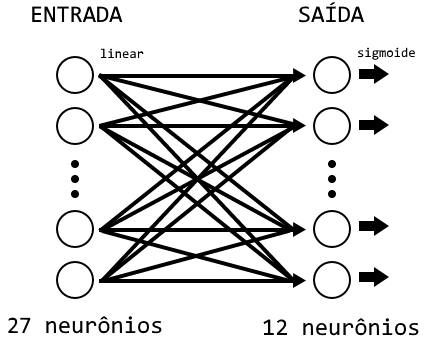
\includegraphics[scale=0.9]{GameNN.png}\\
		\vspace{0.5mm}
		\source{Elaborado pelo autor.}
		\label{fig:gameNN}
	\end{figure}
	
	A camada de entrada possui 33 neurônios,
	que recebem valores entre -1000 e 1000.
	Em sua função de ativação,
	seus valores são multiplicados linearmente por uma constante de 0,002,
	reduzindo o intervalo dos valores para -2 e 2.
	
	A camada de saída possui 12 neurônios,
	e na função de entrada é feito um somatório dos estímulos vindos da camada de entrada multiplicados por um peso.
	Na função de ativação é aplicada a função sigmoide \eqref{eq:sigmoid}
	produzindo saídas no intervalo de 0 a 1
	(ilustrada na Figura \ref{fig:activationFunctions},
	gráfico \textbf{d},
	página \pageref{fig:activationFunctions}).
	
	\begin{equation}
		S(t) = \frac{1}{1 + e^{-t}}
		\label{eq:sigmoid}
	\end{equation}
	
	\vspace{3mm}
	
	A implementação foi feita com o uso de dois vetores e uma matriz,
	sendo que os vetores representam os neurônios da camada de entrada e saída,
	e a matriz é a matriz de pesos da RNA.
	Após o preenchimento do vetor de entrada e a matriz de pesos,
	são feitos os cálculos explicados acima para obter-se o vetor de saída,
	que é o resultado.
	
	\FloatBarrier
	\subsection{Algoritmo Genético Implementado}
	% Tamanho da população
	A população do AG implementado é composta por 40 indivíduos,
	sendo o cromossomo do indivíduo uma matriz de valores reais.
	% População inicializada
	Os genes do cromossomo são inicializados com valores aleatórios entre -1,0 e 1,0.
	
	% Avaliação: cálculo do fitness
	Na avaliação,
	dois indivíduos são selecionados e seus cromossomos
	(que representam a matriz de pesos na RNA)
	são carregados na Rede Neural Artificial.
	Após a execução da RNA em cada comando do jogo,
	é dada uma nota (fitness) sobre a influência que a RNA causou,
	sendo que esta nota pode ser
	positiva se o resultado foi bom,
	ou negativa caso o resultado tenha sido indesejável.
	Mais detalhes sobre os cálculos será mostrado na próxima seção:
	4.4 Funcionamento do jogo.
	
	% Seleção - roleta e montagem da nova população
	% Elitismo
	Após a avaliação de todos os indivíduos da população,
	entra-se no processo de seleção.
	Nesta parte, cria-se a nova população ainda vazia,
	e o objetivo passa a ser preenchê-la até ficar com 40 indivíduos.
	Os primeiros 2 indivíduos que entram nessa nova população são resultado do Elitismo,
	que copia os 2 com melhor fitness da população antiga para lá sem nenhuma modificação.
	
	Para as 38 vagas restantes,
	repete-se o seguinte processo para preenchê-las:
	Primeiro, seleciona-se 2 indivíduos usando o método da Roleta.
	% Crossover (uniforme), taxa
	Após isto, é calculado na taxa de crossover, de 90\%, se haverá crossover ou não.
	Caso haja, é aplicado o crossover uniforme para a geração dos cromossomos filhos,
	que são adicionados na nova população.
	Caso não haja, os indivíduos selecionados são copiados para a nova população.
	
	% Mutação (taxa)
	Na última etapa, a de mutação, a nova população já está preenchida com 40 indivíduos.
	Para cada gene dos 38 cromossomos criados na seleção e crossover,
	é calculada uma chance de 1,5\% de se ocorrer a mutação.
	Se for determinado que haverá uma mutação em um gene,
	haverá uma alteração de 0,3 unidades para mais ou para menos nele,
	escolhido aleatoriamente.
	
	Finalizada a mutação,
	a nova população se torna a população atual e retorna-se na Avaliação,
	repetindo o processo.
	
	\FloatBarrier
	\subsection{Funcionamento do jogo}
	Visto a descrição das variáveis do jogo na seção 4.1
	e a explicação da implementação da Rede Neural Artificial e Algoritmo Genético nas seções 4.2 e 4.3,
	será explicado aqui como cada uma destas partes foram juntadas umas nas outras para formarem o todo,
	%que é um jogo jogado por uma Inteligência Artificial capaz de aprender e mostrar bons resultados.
	que é o trabalho desenvolvido.
	
	\subsubsection{Preparação da batalha}
	% Abertura do jogo pela primeira vez
	Ao abrir o jogo pela primeira vez,
	% criação da população e salvando os dados num arquivo (é salvo junto com a informação de quem já foi avaliado ou não)
	o script do Algoritmo Genético cria uma população aleatória e a salva em um arquivo.
	% Caso tenha fechado o jogo e aberto de novo, as informaçõoes são carregadas de arquivo.
	Desta forma, caso o jogo seja fechado e aberto novamente,
	as informações da população são carregadas do arquivo.
	Neste arquivo são salvos o número que representa a geração atual
	e informações de cada indivíduo da população: os cromossomos, seu fitness e se o cromossomo já foi avaliado.
	
	% Primeiros 2 tem seus cromossomos carregados na RNA, uma para cada time
	Após a população ter sido criada ou carregada,
	procura-se os dois primeiros indivíduos que ainda não foram avaliados.
	Ao encontrar, a informação de seus cromossomos é carregada na matriz de pesos de uma RNA.
	Nesta parte, cada RNA representará a inteligência de um time,
	que por sua vez "emula"{} um jogador real.
	
	\subsubsection{Durante a batalha}
	% Inicia-se a batalha, procura-se o primeiro a receber turno
	Ao iniciar a batalha, cada time tem uma RNA que a representa e controla.
	% O que recebeu turno roda a RNA respectiva a seu time
	O personagem que receber o turno é o que poderá efetuar um comando,
	e neste momento o script de Rede Neural do seu time entra em ação 6 vezes,
	uma para cada diferente personagem ainda em batalha.
	
	% Explicar quais são os valores de entrada que estão sendo usadas na camada de entrada
	Em cada execução da Rede Neural, são usadas como entrada alguns parâmetros do personagem que possuí o turno,
	e parâmetros do possível alvo.
	As informações usadas como entrada na RNA estão descritas na Tabela \ref{tab:nnInput}.
	
	\begin{table}[h]
		\caption{Valores de entrada na RNA}
		\centering
		\small
		\renewcommand{\arraystretch}{1.2} % Aumenta espaçamento vertical
		\begin{tabular}{c|c|c|c}
			\hline 
			\textbf{Atacante}			& \multicolumn{2}{c|}{\textbf{Possível alvo}}	& \textbf{Outros}		\\\hline
			MP usado					& HP perdido		& Def. Física*		& Itens disponíveis* (6)		\\ 
			ATK							& MP usado			& Def. Água*		& Alvo é inimigo?				\\ 
			MAG							& ATK				& Def. Fogo*		& 								\\ 
			SPD							& DEF				& Def. Terra*		& 								\\ 
			Elem. Hab. Fraca* (5)		& MAG				& Def. Vento*		& 								\\ 
			Elem. Hab. Forte* (5)		& RES									& 								\\
										& SPD									& 								\\\hline
		\end{tabular}\\
		\vspace{3mm}
		\source{Elaborado pelo autor.}
		\label{tab:nnInput}
	\end{table}
	
	% Explicação em detalhes de cada entrada na RNA
	No total são 33 entradas,
	em que os que foram marcados com um (X), sendo X um número,
	significa que aquele atributo ainda foi quebrado em X neurônios diferentes.
	No caso da habilidade,
	é subdividido em 5 neurônios para que cada um simbolize um elemento.
	Já nos itens disponíveis,
	são usados 6 neurônios por causa da existência de 6 diferentes itens.
	
	Valores na tabela que contém um * (asterisco) representa que eles tem valor binário.
	Foi implementado que caso o valor seja "falso"{}, "não"{} ou "fraco"{}, terá o valor de -1000.
	Por outro lado, se o valor for "verdadeiro"{}, "sim"{} ou "forte"{}. terá o valor de 1000.
	
	Os demais valores vem com intervalo de 0 a 1000,
	mas que são convertidos para um intervalo de -1000 a 1000,
	ficando no mesmo padrão que as outras entradas.
	Como já visto na seção 4.2,
	o intervalo de -1000 a 1000 é multiplicado por uma constante para se reduzir ao intervalo de -2 a 2.
	
	% Explicar que cada valor de saída siginifica um comando e a chance de usar ele
	Após inserir esses dados nos neurônios de entrada da RNA da equipe,
	é possível fazer os cálculos para se obter seus dados de saída,
	composto por 12 neurônios.
	
	Como já explicado, as saídas tem valores entre 0 e 1.
	A saída do primeiro neurônio é a que calcula a probabilidade daquele personagem se tornar alvo.
	Quanto mais próximo de 1, maior a probabilidade,
	e quanto mais próximo de 0, menor.
	Os outros 11 neurônios representam, cada um, a probabilidade de utilizar um determinado comando naquele personagem, caso ele vire alvo.
	O papel de cada neurônio de saída está ilustrada na Tabela \ref{tab:nnOutput}.
	
	\begin{table}[h]
		\caption{Significado dos valores de saída da RNA}
		\centering
		\small
		\renewcommand{\arraystretch}{1.2} % Aumenta espaçamento vertical
		\begin{tabular}{c|c|c}
			\thickhline 
			\textbf{Alvo}				& \textbf{Atacar}						& \textbf{Defender}				\\\hline
			Prob. de virar alvo			& Prob. de atacar						& Prob. de defender				\\\thickhline
			\textbf{Habilidade}			& 					\multicolumn{2}{c}{\textbf{Usar item}}				\\\hline
			Prob. usar a fraca			& Prob. item dano físico				& Prob. item dano terra			\\ 
			Prob. usar a forte			& Prob. item dano água					& Prob. item dano vento			\\ 
			Prob. usar a cura			& Prob. item dano fogo					& Prob. item poção				\\\thickhline
		\end{tabular}\\
		\vspace{3mm}
		\source{Elaborado pelo autor.}
		\label{tab:nnOutput}
	\end{table}
	
	Então, na verificação de um personagem,
	tem-se a probabilidade dele se tornar alvo e as 11 probabilidades de comandos para utilizar nele.
	Para utilizar esses dados,
	foi criada uma estrutura que une "alvo"{} a "comando"{} em uma única probabilidade,
	se segue a fórmula \eqref{eq:targetCommand} a seguir:
	
	\begin{equation}
		Probabilidade = 1,5 \times Prob. de virar alvo + Prob. comando
		\label{eq:targetCommand}
	\end{equation}
	
	\vspace{3mm}
	
	Desta forma, cria-se 11 combinações de alvo + comando em um personagem.
	Repetindo este processo nos $N$ personagens ainda em batalha,
	obtêm-se $11 \times N$ combinações de alvo e comando no final.
	
	Com todas estas possibilidades em mãos,
	é feita uma ordenação delas de forma que a maior fique em primeiro.
	% Verificação se é viável efetuar o comando (item ou disponível)
	Neste momento,
	o jogo tenta executar a melhor combinação de alvo e comando.
	Caso falhe (por falta de item ou MP),
	tenta-se executar o próximo comando da lista.
	% Efetua-se o comando
	Repete-se as tentativas até que consiga executar algum com sucesso.
	
	% Feedback do comando para avaliação (fitness)
	% Bônus no fitness por derrotar (mostrar fórmula)
	% Repete-se o processo até a batalha acabar
	% Condições de parada: time derrotado ou limite de turnos
	
	\subsubsection{Após a batalha}
	% Finalizada a batalha, fitness das 2 populações são enviadas para o AG e salvas em arquivo
	% Carrega-se os 2 próximos e faz tudo novamente.
	% Após avaliar a população inteira, continuar no processo do AG para gerar a próxima geração, e repete tudo novamente
	

% DESENVOLVIMENTO - FIM

% CONCLUSÃO - INÍCIO
\FloatBarrier
\newpage % Coloca o conteúdo numa nova página
\section{RESULTADOS}
	<Inserir gráficos de evolução do algoritmo, imagens do jogo, explicar desempenho da aprendizagem, etc.>
% CONCLUSÃO - FIM

\FloatBarrier
\newpage % Coloca o conteúdo numa nova página
\section*{\hfil REFERÊNCIAS}
\addcontentsline{toc}{section}{REFERÊNCIAS} % Adiciona as referências no Sumário
	\singlespace
	UNITY. Game engine, tools and multiplatform. 2016a. Disponível em: \textless \url{https://unity3d.com/pt/unity}\textgreater. Acesso em 01 Julho 2016.\par
	UNITY. Made with Unity - Games. 2016b. Disponível em: \textless \url{https://madewith.unity.com/games}\textgreater. Acesso em 01 Julho 2016.\par
	UNITY. Made with Unity - Manual: Learning the Interface. 2016c. Disponível em: \textless \url{https://docs.unity3d.com/Manual/LearningtheInterface.html}\textgreater. Acesso em 05 Julho 2016.\par
	UNITY. Made with Unity - Manual: Creating and Using Scripts. 2016d. Disponível em: \textless \url{https://docs.unity3d.com/Manual/CreatingAndUsingScripts.html}\textgreater. Acesso em 05 Julho 2016.\par
	RIVAL THEORY. Features. 2015. Disponível em: \textless \url{http://rivaltheory.com/rain/features/}\textgreater. Acesso em 01 Julho 2016.\par
	MICROSOFT. Free Dev Tools - Visual Studio Community 2015. 2016. Disponível em: \textless \url{https://www.visualstudio.com/en-us/products/visual-studio-community-vs.aspx}\textgreater. Acesso em 07 Julho 2016.\par
	CNBC. Digital gaming sales hit record \$61 billion in 2015: Report. Disponível em: \textless \url{http://www.cnbc.com/2016/01/26/digital-gaming-sales-hit-record-61-billion-in-2015-report.html}\textgreater. Acesso em 11 Julho 2016.\par
	YANNAKAKIS, Georgios N; TOGELIUS, Julian. A Panorama of Artificial and Computational Intelligence in Games. Disponível em: \textless \url{http://julian.togelius.com/Yannakakis2014Panorama.pdf}\textgreater. Acesso em 11 Julho 2016.\par
	AIGAMEDEV. Top 10 Most Influential AI Games. Disponível em: \textless \url{http://aigamedev.com/open/highlights/top-ai-games/}\textgreater. Acesso em 12 Julho 2016.\par
	ORKIN, Jeff. Three States and a Plan: The A.I. of F.E.A.R. Disponível em: \textless \url{http://alumni.media.mit.edu/~jorkin/gdc2006_orkin_jeff_fear.pdf}\textgreater. Acesso em 12 Julho 2016.\par
	STACKEXCHANGE. How to choose the number of hidden layers and nodes in a feedforward neural network?. Disponível em: \textless \url{https://stats.stackexchange.com/questions/181/how-to-choose-the-number-of-hidden-layers-and-nodes-in-a-feedforward-neural-netw}\textgreater. Acesso em 13 Julho 2016.\par
	STACKEXCHANGE. What does the hidden layer in a neural network compute?. Disponível em: \textless \url{https://stats.stackexchange.com/questions/63152/what-does-the-hidden-layer-in-a-neural-network-compute}\textgreater. Acesso em 13 Julho 2016.\par
	STACKOVERFLOW. Role of Bias in Neural Networks. Disponível em: \textless \url{https://stackoverflow.com/questions/2480650/role-of-bias-in-neural-networks}\textgreater. Acesso em 13 Julho 2016.\par
	OBITKO, Marek. Introduction to Genetic Algorithms. Disponível em: \textless \url{http://www.obitko.com/tutorials/genetic-algorithms/index.php}\textgreater. Acesso em 13 Julho 2016.\par
	RESEARCHGATE. How to select the best transfer function for a neural network model?. Disponível em: \textless \url{https://www.researchgate.net/post/How_to_select_the_best_transfer_function_for_a_neural_network_model}\textgreater. Acesso em 13 Julho 2016.\par
	Wikimedia. File:Colored neural network.svg. Disponível em: \textless \url{https://commons.wikimedia.org/wiki/File:Colored_neural_network.svg}\textgreater. Acesso em 13 Julho 2016.\par
	STACKOVERFLOW. How do you decide the parameters of a Convolutional Neural Network for image classification?. Disponível em: \textless \url{https://stackoverflow.com/questions/24509921/how-do-you-decide-the-parameters-of-a-convolutional-neural-network-for-image-cla}\textgreater. Acesso em 13 Julho 2016.\par
	Tech-Effigy. The Genetic Algorithm - Explained. Disponível em: \textless \url{https://techeffigytutorials.blogspot.com.br/2015/02/the-genetic-algorithm-explained.html}\textgreater. Acesso em 14 Julho 2016.\par
	Evo-neural-network-agents. Simulation of evolution of neural network driven agents in the small world with the pieces of food. Disponível em: \textless \url{https://github.com/lagodiuk/evo-neural-network-agents}\textgreater. Acesso em 14 Julho 2016.\par
	Turing Finance. 10 misconceptions about Neural Networks. Disponível em: \textless \url{http://www.turingfinance.com/misconceptions-about-neural-networks/}\textgreater. Acesso em 14 Julho 2016.\par
	BRAINZ. 15 Real-World Uses of Genetic Algorithms. Disponível em: \textless \url{http://brainz.org/15-real-world-applications-genetic-algorithms/}\textgreater. Acesso em 20 Julho 2016.\par
	STACKOVERFLOW. Genetic Programming : Difference between Roulette Rank and Tournament Selection. Disponível em: \textless \url{https://stackoverflow.com/questions/23183862/genetic-programming-difference-between-roulette-rank-and-tournament-selection}\textgreater. Acesso em 20 Julho 2016.\par
	Wikipedia. File:Logistic-curve.svg. Disponível em: \textless \url{https://en.wikipedia.org/wiki/File:Logistic-curve.svg}\textgreater. Acesso em 13 Julho 2016.\par

\end{document}
